\subsection{Process Scheduling}\label{subsec:Process_Scheduling}
With multiprogramming, the objective is to have \textbf{some} \nameref{def:Process} running at all times.
Note that we are discussing a computer with a single CPU, and likely a single \nameref{def:Thread} here.
Time sharing makes the CPU \nameref{def:Context_Switch} so frequently that users can interact with each program and it seems like they are all running concurrently.

\begin{definition}[Process Scheduler]\label{def:Process_Scheduler}
  The \emph{process scheduler} is responsible for selecting an available process (one in the New, Ready, or Running states discussed in \Cref{subsubsec:Process_States}) from one of possibly many queues to run next.
\end{definition}

\subsubsection{Scheduling Queues}\label{subsubsec:Scheduling_Queues}
When a \nameref{def:Process} enters the system, it is put in the \textbf{Job Queue}, which consists of \textbf{EVERY} process on the system.

The processes that are in main memory, are ready, and waiting to execute are in the \textbf{Ready Queue}.
The \nameref{def:Process_Control_Block}s are kept in a doubly linked list, with the first and last PCBs explicitly marked by the list itself and a pointer to the next PCB in the ready queue in each PCB.\@

There are other queues as well:
\begin{itemize}[noitemsep]
\item \textbf{Device Queue}: Completion of I/O Request(s)
  \begin{itemize}[noitemsep]
  \item Each device has its own queue.
  \end{itemize}
\end{itemize}

These various queues can be represented by \Cref{fig:Queues}.
\begin{figure}[h!tbp]
  \centering
  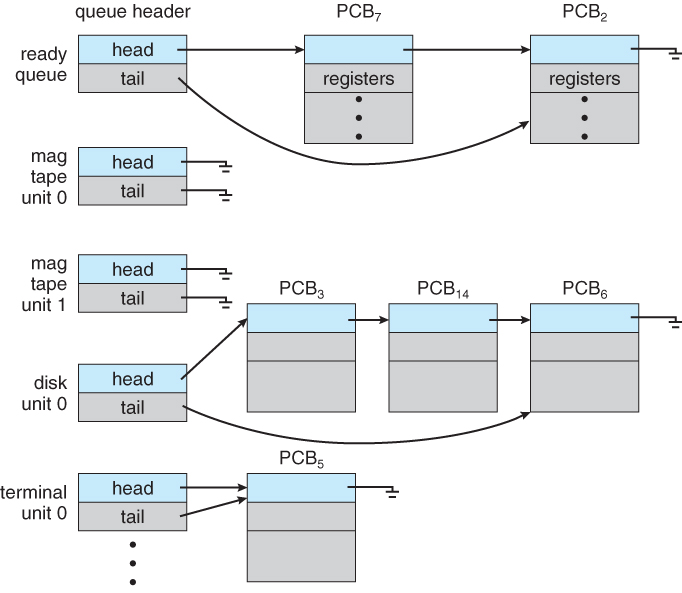
\includegraphics[scale=1.00]{./Drawings/EDAF35-Operating_Systems/Queues.jpg}
  \caption{Various System Queues}
  \label{fig:Queues}
\end{figure}

A good visualization of how \nameref{def:Process}es and their queues work is shown in \Cref{fig:Queuing_Diagram}.

\begin{figure}[h!tbp]
  \centering
  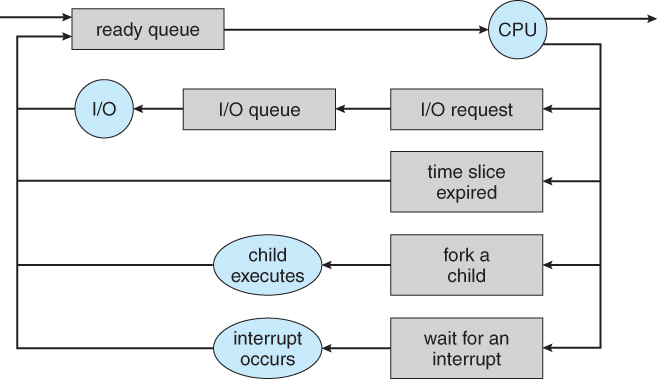
\includegraphics[scale=1.00]{./Drawings/EDAF35-Operating_Systems/Queuing_Diagram.jpg}
  \caption{Queuing Diagram for Process Scheduling}
  \label{fig:Queuing_Diagram}
\end{figure}

\subsubsection{Schedulers}\label{subsubsec:Schedulers}
\begin{definition}[Scheduler]\label{def:Scheduler}
  A \emph{scheduler} is responsible for selecting the \nameref{def:Process} from one of the queues to execute next.
\end{definition}

Typically, many more \nameref{def:Process}es are submitted at once than can be handled immediately.
So, some are sent to a mass-storage device where they are keyp for later scheduling by the \emph{long-term scheduler} or \emph{job scheduler}.
The \emph{short-term scheduler}, or the \emph{CPU scheduler} selects from the \nameref{def:Process}es that are ready to execute and allocates the CPU to them.
The CPU scheduler is run every hundred milliseconds, whereas the job scheduler may be run every few minutes.
This allows the job scheduler to run for longer periods of time, because it is active for less time overall.

The job scheduler determines the \emph{degree of multiprogramming}, by determining how many \nameref{def:Process}es can live in memory at any given time.
If the degree of multiprogramming is stable, then the average rate of process creation must be equal to the average departure rate of processes leaving the system.
Most desktop \nameref{def:Operating_System}s do not use the long-term scheduler.
Instead they put all tasks into the short-term queue, and rely on human behavior to help control the business of the systems.

\begin{definition}[I/O Bound]\label{def:IO_Bound}
  An \emph{I/O Bound} \nameref{def:Process} is one where most of the process's time is spent performing I/O rather than computations.
\end{definition}

\begin{definition}[CPU-Bound]\label{def:CPU_Bound}
  A \emph{CPU-Bound} \nameref{def:Process} spends most of its time performing computations.
\end{definition}

It is important to have a good mix of \nameref{def:IO_Bound} and \nameref{def:CPU_Bound} processes, so that no single queue is ever too full, improving overall system throughput.

There are also \emph{medium-term scheduler}s that perform \emph{swapping}.
This scheduler removes a \nameref{def:Process} from memory, store it somewhere, then reintroduce the process to memory again later.

%%% Local Variables:
%%% mode: latex
%%% TeX-master: "../../EDAF35-Operating_Systems-Reference_Sheet"
%%% End:
